%%
%% Copyright 2026 Oxford University Press
%%
%%
%% v1.3 released March 2026
%%
%% This file is part of the 'pnas-nexus-authoring-template Bundle'.
%% ---------------------------------------------
%%
%% It may be distributed under the conditions of the LaTeX Project Public
%% License, either version 1.2 of this license or (at your option) any
%% later version.  The latest version of this license is in
%%    http://www.latex-project.org/lppl.txt
%% and version 1.2 or later is part of all distributions of LaTeX
%% version 1999/12/01 or later.
%%
%% The list of all files belonging to the 'pnas-nexus-authoring-template Bundle' is
%% given in the file `manifest.txt'.
%%
%% Template article for PNAS Nexus's document class `oup-authoring-template'
%% with bibliographic references
%%
%%
%% Change log
%%
%% v1.0 2021
%%    Adapted from oup_authoring_template.cls for use with pnas-nexus-authoring-template.tex
%% v1.1 August 2024
%%    Adjusted text of copyright statement for use with pnas-nexus-authoring-template.tex
%% v1.2 January 2025
%%    Updated journal logo
%% v1.3 March 2026
%%    Updated page design


\documentclass[unnumsec,webpdf,modern,large]{oup-authoring-template}%
%\onecolumn % for one column layouts
\usepackage{tikz}
\usepackage{booktabs}
\usepackage[T1,T5]{fontenc}
\usepackage[utf8]{inputenc}
\usetikzlibrary{shapes.geometric, arrows.meta, positioning}

%\usepackage{showframe}

\graphicspath{{Fig/}}
\def\societylogo{}

% line numbers
%\usepackage[mathlines, switch]{lineno}
%\usepackage[right]{lineno}

\theoremstyle{thmstyleone}%
\newtheorem{theorem}{Theorem}%  meant for continuous numbers
%%\newtheorem{theorem}{Theorem}[section]% meant for sectionwise numbers
%% optional argument [theorem] produces theorem numbering sequence instead of independent numbers for Proposition
\newtheorem{proposition}[theorem]{Proposition}%
%%\newtheorem{proposition}{Proposition}% to get separate numbers for theorem and proposition etc.
\theoremstyle{thmstyletwo}%
\newtheorem{example}{Example}%
\newtheorem{remark}{Remark}%
\theoremstyle{thmstylethree}%
\newtheorem{definition}{Definition}

\begin{document}

\journaltitle{} 
\DOI{DOI added during production}
\copyrightyear{2026}
\pubyear{2026}
\vol{0} 
\issue{0}
\access{Published: Date added during production}
\appnotes{Paper}

\firstpage{1}

%\subtitle{Subject Section}

\title[Contextual extraction with a LoRA-fine-tuned LM]{Contextual information extraction of customer data from sales audio calls using a LoRA-fine-tuned language model}

\author[1]{Thomas Hoang}

\address[1]{\orgname{Student ID: A1984077}}

\received{Date}{0}{2026}
\revised{Date}{0}{2026}
\accepted{Date}{0}{2026}

%\editor{Associate Editor: Name}

\abstract{Sales agents on our CRM platform (uCall) currently fill in customer fields by hand after every call. This project presents a three-stage pipeline to automate that process: (1) Silero VAD removes silence and noise from the raw audio, (2) a wav2vec\,2.0 model transcribes the remaining speech in Vietnamese, and (3) a LoRA-fine-tuned LLM extracts structured CRM fields from the transcript. The full staging export comprises 13{,}232 manual sales calls. An initial evaluation subset of 600 calls was selected; after dropping 50 broken records that failed to yield transcripts, the final dataset comprises 550 calls. This dataset uses an 80/20 train--test split (440 train, 110 test) for the extraction stage. Evaluation uses Word Error Rate for ASR and field-level metrics on the held-out test set (JSON validity and agreement with teacher labels).} 

\keywords{keyword1, keyword2, keyword3, keyword4}

\keywords[Abbreviations]{abbreviation1, abbreviation2, abbreviation3, abbreviation4}

\otherabstract[Significance statement]{Research reports require a significance statement of between 50 and 120 words. Abbreviations are permitted, but citations cannot be included. If required, un-comment this element in the template to include. The heading is included automatically.}

\maketitle
\thispagestyle{empty}

%\begin{epigraph}
%Epigraph text. Ximporem qui reperov idempedit modio. Bisto imagnatem quae aceptis
%nobitae quid eum rae adignis quias-sit vellacc uptatur sunt quis rentis eaquasit alia deliquam
%rec-to consed unt. Empor sum ratur ressimusdae. Nam fugiae.
%\source{Epigraph source}
%\end{epigraph}

% =============================================================================
% PLACEHOLDER --- delete this entire section before final submission / export.
% =============================================================================
\section*{Scope and assumptions agreement \textit{(draft placeholder---remove later)}}
\label{sec:scope-agreement-placeholder}

\noindent\textit{This section is for supervisor/student alignment only. It is not part of the final paper. Delete everything from here through the horizontal rule below once scope, data, methods, and evaluation are agreed.}

\subsection*{Purpose}
Decisions to lock before drafting, so every section of the report (Introduction $\rightarrow$ Conclusion) uses the \emph{same} numbers, names, and claims. For each item, mark the chosen answer; anything left as \textbf{TBD} blocks writing that section.

\subsection*{A. Global consistency (must match in every section, abstract, and figures)}
\begin{enumerate}
  \item[A1.] Project title / one-line problem statement --- final wording?
  \item[A2.] Product name spelling and casing (``uCall'') used everywhere?
  \item[A3.] Corpus numbers: full $=13{,}232$; initial $=600$; dropped $=50$; used $=550$; split $=440$ train $/$ $110$ test --- frozen for all sections?
  \item[A4.] Canonical stage names: ``VAD'', ``ASR'', ``Contextual Extraction'' --- fixed labels and order?
  \item[A5.] CRM field list + types (\texttt{customer\_sector}, \texttt{customer\_needs}, \texttt{customer\_interested} 1--10, \texttt{customer\_busy} bool, \texttt{customer\_scheduled\_at} date$|$null, \texttt{customer\_rating}) --- final schema?
  \item[A6.] Terminology: ``teacher / student'', ``LoRA'', ``fine-tune'' vs ``distill'' --- pick one vocabulary.
  \item[A7.] Random seeds reported (data split $=42$; training $=3407$) --- state both?
\end{enumerate}

\subsection*{B. Introduction (Sec.~1)}
\begin{enumerate}
  \item[B1.] Motivation framing: business cost of manual entry, or broader ML/ASR+LLM angle, or both?
  \item[B2.] Exactly which 2--3 contributions do we claim? (pipeline / stereo dialogue / LLM-labeled LoRA / deployable API)
  \item[B3.] Do we claim any quantitative headline result in the intro, or keep it qualitative?
\end{enumerate}

\subsection*{C. Related Work + Novelty (Sec.~2)}
\begin{enumerate}
  \item[C1.] Scope of literature: VAD, Vietnamese ASR, small-LLM info-extraction, LLM-as-judge/teacher --- which to include?
  \item[C2.] Stated gap we address (e.g.\ end-to-end Vietnamese telesales $\rightarrow$ CRM JSON with small local models)?
  \item[C3.] Novelty claim wording --- is it ``novel system/application'' rather than ``novel algorithm''? Agree honestly.
\end{enumerate}

\subsection*{D. Methodology (Sec.~3)}
\begin{enumerate}
  \item[D1.] System diagram: include? what blocks/arrows? who produces it?
  \item[D2.] Which equations are required (CE loss over response tokens, LoRA $\Delta W = BA$, attention, WER)?
  \item[D3.] Depth on ASR: describe deployed service as black box, or include model internals?
  \item[D4.] Prompt/label schema shown verbatim (the Gemini extraction prompt)?
\end{enumerate}

\subsection*{E. Experimental Setup (Sec.~4)}
\begin{enumerate}
  \item[E1.] Data subsection: SQL filter, duration rule, dedup, language --- what to disclose?
  \item[E2.] Train/val/test --- do we add a validation set or keep train/test only? Justify.
  \item[E3.] Hardware/software: exact GPU (Colab T4/A100?), PyTorch + Unsloth + bitsandbytes versions?
  \item[E4.] Hyperparameter table contents: $r{=}16$, $\alpha{=}16$, dropout $0$, lr $2\mathrm{e}{-4}$, batch $2$, grad-accum $4$, epochs $1$, max-seq $2048$, 4-bit --- added table.
  \item[E5.] Which models actually trained/reported (\texttt{Qwen/Qwen3.5-2B}, \texttt{Qwen/Qwen3.5-0.8B}, \texttt{google/gemma-4-E4B} [failed at training])?
\end{enumerate}

\subsection*{F. Results (Sec.~5)}
\begin{enumerate}
  \item[F1.] Baseline definition: base (non-fine-tuned) model? Gemini upper bound? trivial majority class?
  \item[F2.] Final metric set: WER (ASR) + Valid JSON \%, busy acc, sector/schedule match, interested/rating MAE --- and do we add Precision/Recall/F1?
  \item[F3.] Required figures: loss curve, per-field bar chart, call-duration histogram, VAD before/after --- which make the cut?
  \item[F4.] Honesty on the earlier no-split bug --- report corrected numbers only, or show before/after?
\end{enumerate}

\subsection*{G. Discussion (Sec.~6, highest weight)}
\begin{enumerate}
  \item[G1.] Which ``war stories'' to tell (forgot train/test split; rate-limited Gemini labeling; stereo vs mono; resampling; checkpoint/resume)?
  \item[G2.] Key learnings to highlight (teacher-bias ceiling, small-model viability, data quality $>$ size)?
  \item[G3.] Future directions (2--3): scale to 13k, human-audited labels, streaming/real-time ASR, multi-tenant CRM schema?
\end{enumerate}

\subsection*{H. Conclusion (Sec.~7) + formatting}  
\begin{enumerate}
  \item[H1.] Single headline takeaway sentence?
  \item[H2.] Template/format final: this OUP/PNAS style, or switch to NeurIPS/ICLR? Page limit?
  \item[H3.] Citation style + reference manager (BibTeX \texttt{reference.bib}); cite datasets, HF models, libraries?
  \item[H4.] Anonymisation / data-availability statement wording (internal data --- can it be shared?).
\end{enumerate} 
 
\noindent\textbf{Agreed by:} Student \underline{\hspace{4cm}} \quad Supervisor \underline{\hspace{4cm}} \quad Date \underline{\hspace{3cm}}

\vspace{1em}   
\noindent\rule{\textwidth}{0.4pt}
\smallskip
\noindent\textit{End of placeholder section --- remove everything above this line before submission.}
% =============================================================================

\clearpage

% -----------------------------------------------------------------------------
% Assignment report outline (sections 1--7, titles only)
% -----------------------------------------------------------------------------
\makeatletter
\@unnumsecfalse
\makeatother
\setcounter{secnumdepth}{2}

\section{Introduction}
\label{sec:introduction}

\subsection{Problem Statement} 
Sales agents on the uCall platform currently fill in customer data fields by hand after every call. This manual process takes too much time and causes errors. We are building an automated system to extract structured CRM fields directly from raw audio calls.

\subsection{Motivation}
Manual data entry costs businesses time and money. Large language models can extract this data but they are often too big and expensive to run. This project shows how to combine audio processing tools with a small local language model. We use a fine tuning method called LoRA to accurately extract data using standard hardware. \textbf{This is important because it proves that companies do not need huge external models to automate their data tasks.}

\subsection{Contributions}
\begin{itemize}
    \item Developed a complete and production ready pipeline to process raw audio into structured data.
    \item (Placeholder) I will add the quantitative results later.
    \item Deployed a fine tuned local language model that extracts data without relying on expensive cloud APIs.
\end{itemize}

\section{Related Work} 
\label{sec:related-work}
Information extraction from spoken dialogue combines speech recognition and language modeling. Existing methods often rely on huge language models for zero shot extraction like ChatGPT \cite{wei2023zero_shot_ie} or use separate large scale speech models like Whisper \cite{whisper_repo}. While these approaches are accurate they are very expensive and slow for business use. Other research focuses on base architectures \cite{vaswani2017attention} or audio models like wav2vec 2.0 \cite{baevski2020wav2vec2} and Zipformer \cite{zipformer_paper}. However most studies look at these models in isolation. The gap in the current literature is a lack of end to end systems optimized for specific tasks on cheap hardware. Our approach combines a Vietnamese wav2vec 2.0 model with a small local language model. We use LoRA \cite{hu2022lora} to train this small model to perform extraction as well as massive models.

\subsection{Novelty and Significance}
This project is novel because it \textbf{builds a complete pipeline from raw stereo audio to structured data without relying on huge external APIs}. We use Silero VAD \cite{SileroVAD} to clean the audio and maintain speaker channels. Then we \textbf{fine tune a small local model to replace expensive cloud services}. The significance of this work is that it \textbf{provides a practical blueprint for companies to automate data entry}. It shows that businesses can \textbf{achieve high accuracy on domain specific tasks using local hardware}.

\section{Methodology} 
\label{sec:methodology} 

The goal of this work is to automatically extract customer information from call audio and fill the CRM fields. We propose a three-stage pipeline to accomplish this, as illustrated in Figure~\ref{fig:pipeline}. 

\begin{figure}[hbt!]
  \centering
  \resizebox{0.6\linewidth}{!}{
  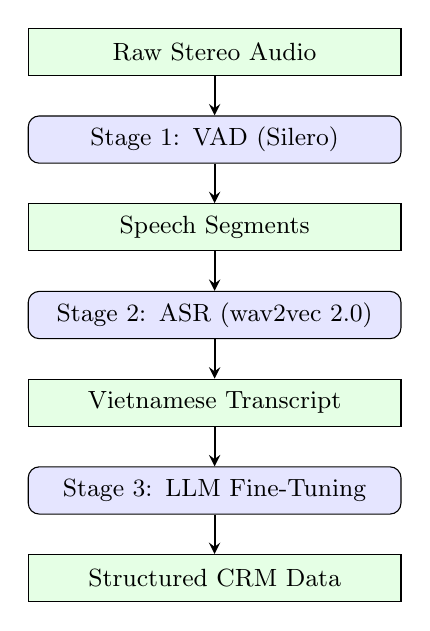
\begin{tikzpicture}[
      node distance=0.5cm,
      block/.style={rectangle, draw, fill=blue!10, text width=4.5cm, text centered, rounded corners, minimum height=0.6cm, font=\small},
      data/.style={rectangle, draw, fill=green!10, text width=4.5cm, text centered, minimum height=0.6cm, font=\small},
      arrow/.style={thick,->,>=stealth}
    ]
    \node [data] (audio) {Raw Stereo Audio};
    \node [block, below=of audio] (vad) {Stage 1: VAD (Silero)};
    \node [data, below=of vad] (segments) {Speech Segments};
    \node [block, below=of segments] (asr) {Stage 2: ASR (wav2vec 2.0)};
    \node [data, below=of asr] (transcript) {Vietnamese Transcript};
    \node [block, below=of transcript] (llm) {Stage 3: LLM Fine-Tuning};
    \node [data, below=of llm] (json) {Structured CRM Data};
    
    \draw [arrow] (audio) -- (vad);
    \draw [arrow] (vad) -- (segments);
    \draw [arrow] (segments) -- (asr);
    \draw [arrow] (asr) -- (transcript);
    \draw [arrow] (transcript) -- (llm);
    \draw [arrow] (llm) -- (json);
  \end{tikzpicture}
  }
  \caption{The three-stage contextual extraction pipeline.}
  \label{fig:pipeline}
\end{figure}

\subsection{Stage 1: Voice Activity Detection (VAD)} 
Raw files contain silence, hold tones, background noise, and non-speech events, which increase speech recognition errors. Preprocessing limits those segments. Recordings are stereo, with the agent on the left channel and the customer on the right. Since downstream analysis targets the customer, we isolate the right channel before VAD. 

We reviewed comparative VAD evidence on mixed-domain audio at 16\,kHz \cite{SileroVADQualityMetrics}. In that evaluation, \textbf{Silero v6} reports the best multi-domain ROC-AUC (\textbf{0.97}) and high chunk-level speech accuracy (\textbf{0.92}). Based on this quality evidence and deployment constraints, we adopted \textbf{Silero VAD} for this pipeline \cite{SileroVAD,SileroVADQualityMetrics}. We retain the speech intervals and drop the rest, removing long silent regions and background sound prior to ASR. Figure~\ref{fig:vad_before_after} shows an example call before and after VAD processing.
 
\begin{figure}[hbt!] 
  \centering
  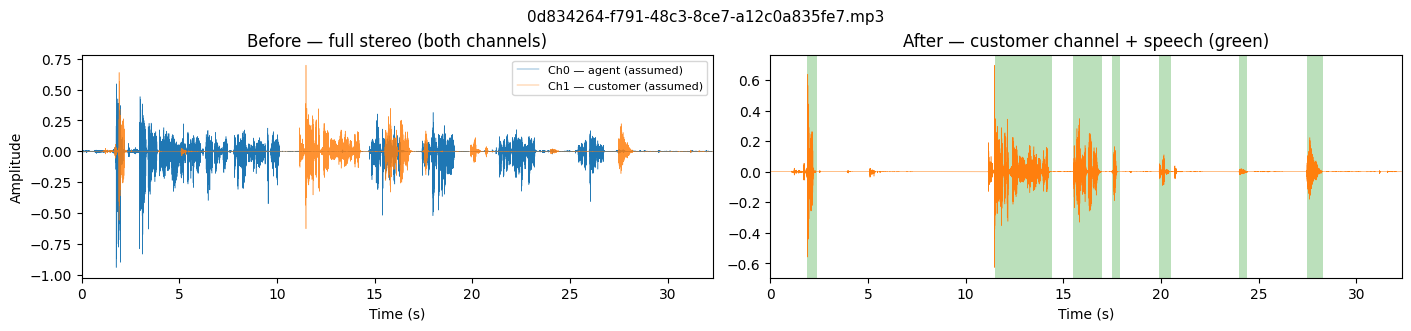
\includegraphics[width=\linewidth]{images/before_after_process_vad.png}
  \caption{One call: stereo mix (left) and customer channel with VAD speech regions (right).}
  \label{fig:vad_before_after}
\end{figure}

\subsection{Stage 2: Automatic Speech Recognition (ASR)}
After VAD segmentation, each speech-only chunk is forwarded to an Automatic Speech Recognition (ASR) model to convert audio segments into unstructured text transcripts. The segment transcripts are then merged by timestamp to reconstruct the full-call transcript. 

Three ASR candidates were considered: wav2vec 2.0 with a Vietnamese checkpoint \cite{nguyenvulebinh_wav2vec2_base_vi}, Whisper \cite{whisper_repo}, and Zipformer \cite{zipformer_hf,zipformer_paper}. Ultimately, we chose the wav2vec 2.0 model (\texttt{nguyenvulebinh/wav2vec2-base-vi}) because it has already been running reliably in our production environment for 1.5 years.

In a real-world startup environment, practical constraints often matter just as much as theoretical benchmarks. Relying on a proven, already-integrated model avoids the technical debt and unexpected blockers that can come with migrating to an entirely new architecture. Because of this existing infrastructure, the pipeline implementation does not load the ASR model locally. Instead, it delegates the transcription task by making calls to our internal, containerized API that serves the model.

\subsection{Stage 3: LLM Fine-Tuning}
In the final stage, reconstructed transcripts are formatted into a supervised fine-tuning dataset for a downstream large language model. The model is trained to extract a comprehensive set of customer information in a single pass, outputting a structured JSON object. The target CRM schema contains six specific fields, as detailed in Table~\ref{tab:crm_fields}.

\begin{table}[hbt!]
  \centering
  \caption{CRM JSON Field Schema Extracted by the LLM}
  \label{tab:crm_fields}
  \begin{tabular}{p{0.35\linewidth} p{0.2\linewidth} p{0.4\linewidth}}
    \toprule
    \textbf{Field Name} & \textbf{Data Type} & \textbf{Description} \\
    \midrule
    \texttt{customer\_sector} & String$|$Null & Industry or sector \\
    \texttt{customer\_needs} & String & Brief summary of what the customer needs \\
    \texttt{customer\_interested} & Number & 1--10 scale of interest \\
    \texttt{customer\_busy} & Boolean & True if they said they are busy, false otherwise \\
    \texttt{customer\_scheduled\_at} & String$|$Null & Time or date they want to be called back \\
    \texttt{customer\_rating} & Number$|$Null & Optional 1--10 rating, if available \\
    \bottomrule
  \end{tabular}
\end{table}  
 
Of the initial 600 selected calls, 50 records were dropped because they failed to generate a transcript during the ASR stage. The remaining dataset is compiled into 550 rows of JSON-formatted training examples for supervised fine-tuning. Each row contains the \texttt{instruction} (the extraction prompt and schema), the \texttt{input} (the full call transcript), and the \texttt{response} (the exact JSON output with all six fields populated). A representative training example is shown below (the transcript and response are formatted for readability):

\begin{verbatim} 
{
  "call_id": "03bc8c4e...",
  "instruction": "You are a structured-field 
extractor for telesales CRM QA. Read the  
following transcript and extract the  
customer information.  
Output valid JSON matching this schema exactly: 
{
  \"customer_sector\": \"string\",
  \"customer_needs\": \"string\",
  \"customer_interested\": \"number (1-10)\",
  \"customer_busy\": \"boolean\",
  \"customer_scheduled_at\": \"string or null\",
  \"customer_rating\": \"number (1-10)\"
}
Return only JSON. Do not include markdown.",
  "input": "[Full Vietnamese call transcript...]",
  "response": "[Extracted values matching schema]"
}
\end{verbatim}

\subsubsection{Model Architecture and Loss}
Candidate model families for extraction initially included:
\begin{itemize}
    \item \texttt{Qwen/Qwen3.5-2B}: Evaluated successfully.
    \item \texttt{Qwen/Qwen3.5-0.8B}: Evaluated successfully.
    \item \texttt{google/gemma-4-E4B}: Excluded from final evaluation (failed during training). 
\end{itemize}

All are decoder-only Transformer models \cite{vaswani2017attention} built on self-attention:
\[
  \mathrm{Attention}(Q,K,V)=\mathrm{softmax}({QK^{\top}}/{\sqrt{d_k}})\,V,
\]
which allows tokens to attend to the full transcript to resolve implicit context. Smaller models are preferred to reduce inference and training costs.

Because updating every parameter of the model is computationally expensive, we employ Low-Rank Adaptation (LoRA) \cite{hu2022lora}. The pre-trained weights are frozen and only a low-rank update is trained, cutting trainable parameters to a small fraction. We train using the standard autoregressive cross-entropy loss over the response tokens:
\begin{equation}
  \mathcal{L} = -\frac{1}{|\mathcal{R}|} \sum_{t \in \mathcal{R}} \log\, p_\theta\!\bigl(y_t \mid y_{<t}\bigr)
  \label{eq:ce_loss}
\end{equation}
where $\mathcal{R}$ is the set of response-token positions. Minimising this loss teaches the model to assign high probability to the exact labels defined by the CRM field configuration.

\section{Experimental Setup}
\label{sec:experimental-setup}

\subsection{Data}
The dataset is extracted from the internal staging database of our organization, consisting of real manual sales calls made through the CRM system. We selected calls with a duration greater than 5 seconds to exclude empty or dropped connections. The full export contains 13,232 stereo audio records. For the purposes of evaluating the extraction pipeline in this project, an initial subset of 600 calls was selected. During processing, 50 records were dropped due to being broken (failing to yield a transcript), resulting in a final curated dataset of 550 calls. This dataset is partitioned into an 80/20 train-test split (440 train, 110 test) for supervised fine-tuning.

\begin{figure}[ht]
\centering
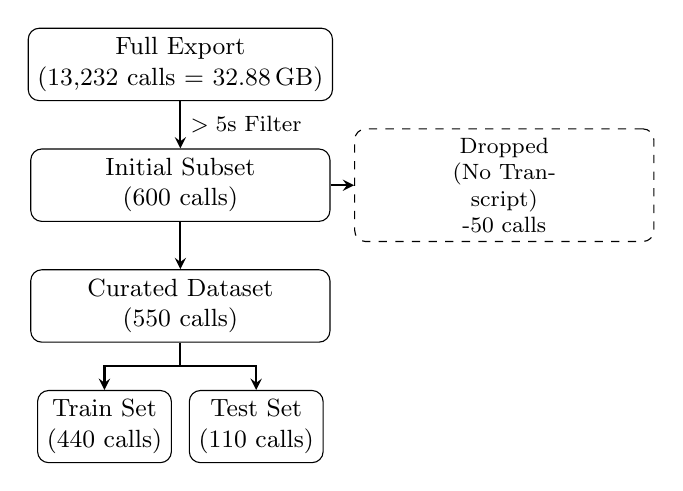
\begin{tikzpicture}[
  box/.style={draw, rectangle, rounded corners, minimum width=3.8cm, minimum height=0.6cm, align=center, font=\small},
  smallbox/.style={draw, rectangle, rounded corners, minimum width=1.6cm, minimum height=0.6cm, align=center, font=\small},
  arrow/.style={thick,->,>=stealth}
]
  \node (full) [box] {Full Export\\(13,232 calls = 32.88\,GB)};
  \node (subset) [box, below=0.6cm of full] {Initial Subset\\(600 calls)};
  \node (dropped) [box, right=0.3cm of subset, dashed, text width=2cm, font=\footnotesize] {Dropped\\(No Transcript)\\{-50 calls}};
  \node (final) [box, below=0.6cm of subset] {Curated Dataset\\(550 calls)};
  \node (train) [smallbox, below left=0.6cm and -1.8cm of final] {Train Set\\(440 calls)};
  \node (test) [smallbox, below right=0.6cm and -1.8cm of final] {Test Set\\(110 calls)};

  \draw [arrow] (full) -- node[right, font=\footnotesize] {$> 5$s Filter} (subset);
  \draw [arrow] (subset) -- (dropped);
  \draw [arrow] (subset) -- (final);
  \draw [arrow] (final.south) -- ++(0,-0.3) -| (train.north);
  \draw [arrow] (final.south) -- ++(0,-0.3) -| (test.north);
\end{tikzpicture}
\caption{Dataset curation and train-test splitting process.}
\label{fig:dataset_flow}
\end{figure}

\subsection{Hardware and Software}
The pipeline is executed across two distinct environments to balance local prototyping and accelerated training:
\begin{itemize}
    \item \textbf{Local Preprocessing (Apple MacBook M4):} Used for the initial data preparation stages, including stereo audio isolation, Voice Activity Detection using Silero VAD (v6.2.1), and assembling the final JSON training dataset.
    \item \textbf{Cloud Training (Google Colab T4):} The computationally intensive supervised fine-tuning (Stage 3) is conducted in the cloud using an NVIDIA T4 GPU (16\,GB VRAM). 
    \item \textbf{Software Stack:} The environment is managed via Conda on Python 3.11.15. Key libraries include PyTorch (v2.11.0) for tensor operations, the Hugging Face \texttt{transformers} library (v5.5.0) for model architectures, and Unsloth for LoRA training.
\end{itemize}

\subsection{Hyperparameters}
To ensure reproducibility, the hyperparameter configuration used for the supervised fine-tuning of the Qwen models is provided in Table \ref{tab:hyperparameters}. We utilized 4-bit quantization alongside Low-Rank Adaptation (LoRA) \cite{hu2022lora} to optimize memory efficiency and fit the training workload within the 16\,GB limit of the T4 GPU.

\begin{table}[h]
\centering
\caption{Model Fine-Tuning Hyperparameters}
\begin{tabular}{@{}ll@{}}
\toprule
\textbf{Hyperparameter} & \textbf{Value} \\
\midrule
LoRA Rank ($r$) & 16 \\
LoRA Alpha ($\alpha$) & 16 \\
LoRA Dropout & 0 \\
Learning Rate & $2 \times 10^{-4}$ \\
Per-Device Batch Size & 2 \\
Gradient Accumulation Steps & 4 \\
Effective Batch Size & 8 \\
Epochs & 1 \\
Max Sequence Length & 2048 tokens \\
Quantization & 4-bit (NF4) \\
\bottomrule
\end{tabular}
\label{tab:hyperparameters}
\end{table}

These specific hyperparameters were chosen to balance model performance against strict hardware limitations and data constraints:
\begin{itemize}
    \item \textbf{Epochs ($1$):} Given the relatively small size of the curated dataset (440 training records), limiting training to a single epoch helps prevent the model from catastrophically overfitting and memorizing the training transcripts.
    \item \textbf{Batch Size ($2$) \& Gradient Accumulation ($4$):} A small per-device batch size was strictly necessary to avoid Out-Of-Memory (OOM) errors on the 16\,GB T4 GPU. Gradient accumulation is used to simulate a larger effective batch size of 8, which stabilizes the training gradients.
    \item \textbf{LoRA Rank ($r{=}16$):} A rank of 16 provides an optimal trade-off between expressivity and memory overhead. It introduces enough trainable parameters to help the model learn the complex JSON extraction schema without inflating VRAM usage.
\end{itemize}

\section{Results}
\label{sec:results}

\subsection{Training Convergence}
Figure \ref{fig:training_loss} illustrates the training loss for both the Qwen3.5-0.8B and Qwen3.5-2B models across the 55 training steps. Both models demonstrate clear convergence, rapidly adapting to the JSON schema format and stabilizing towards the end of the single epoch. 

\begin{figure}[h]
    \centering
    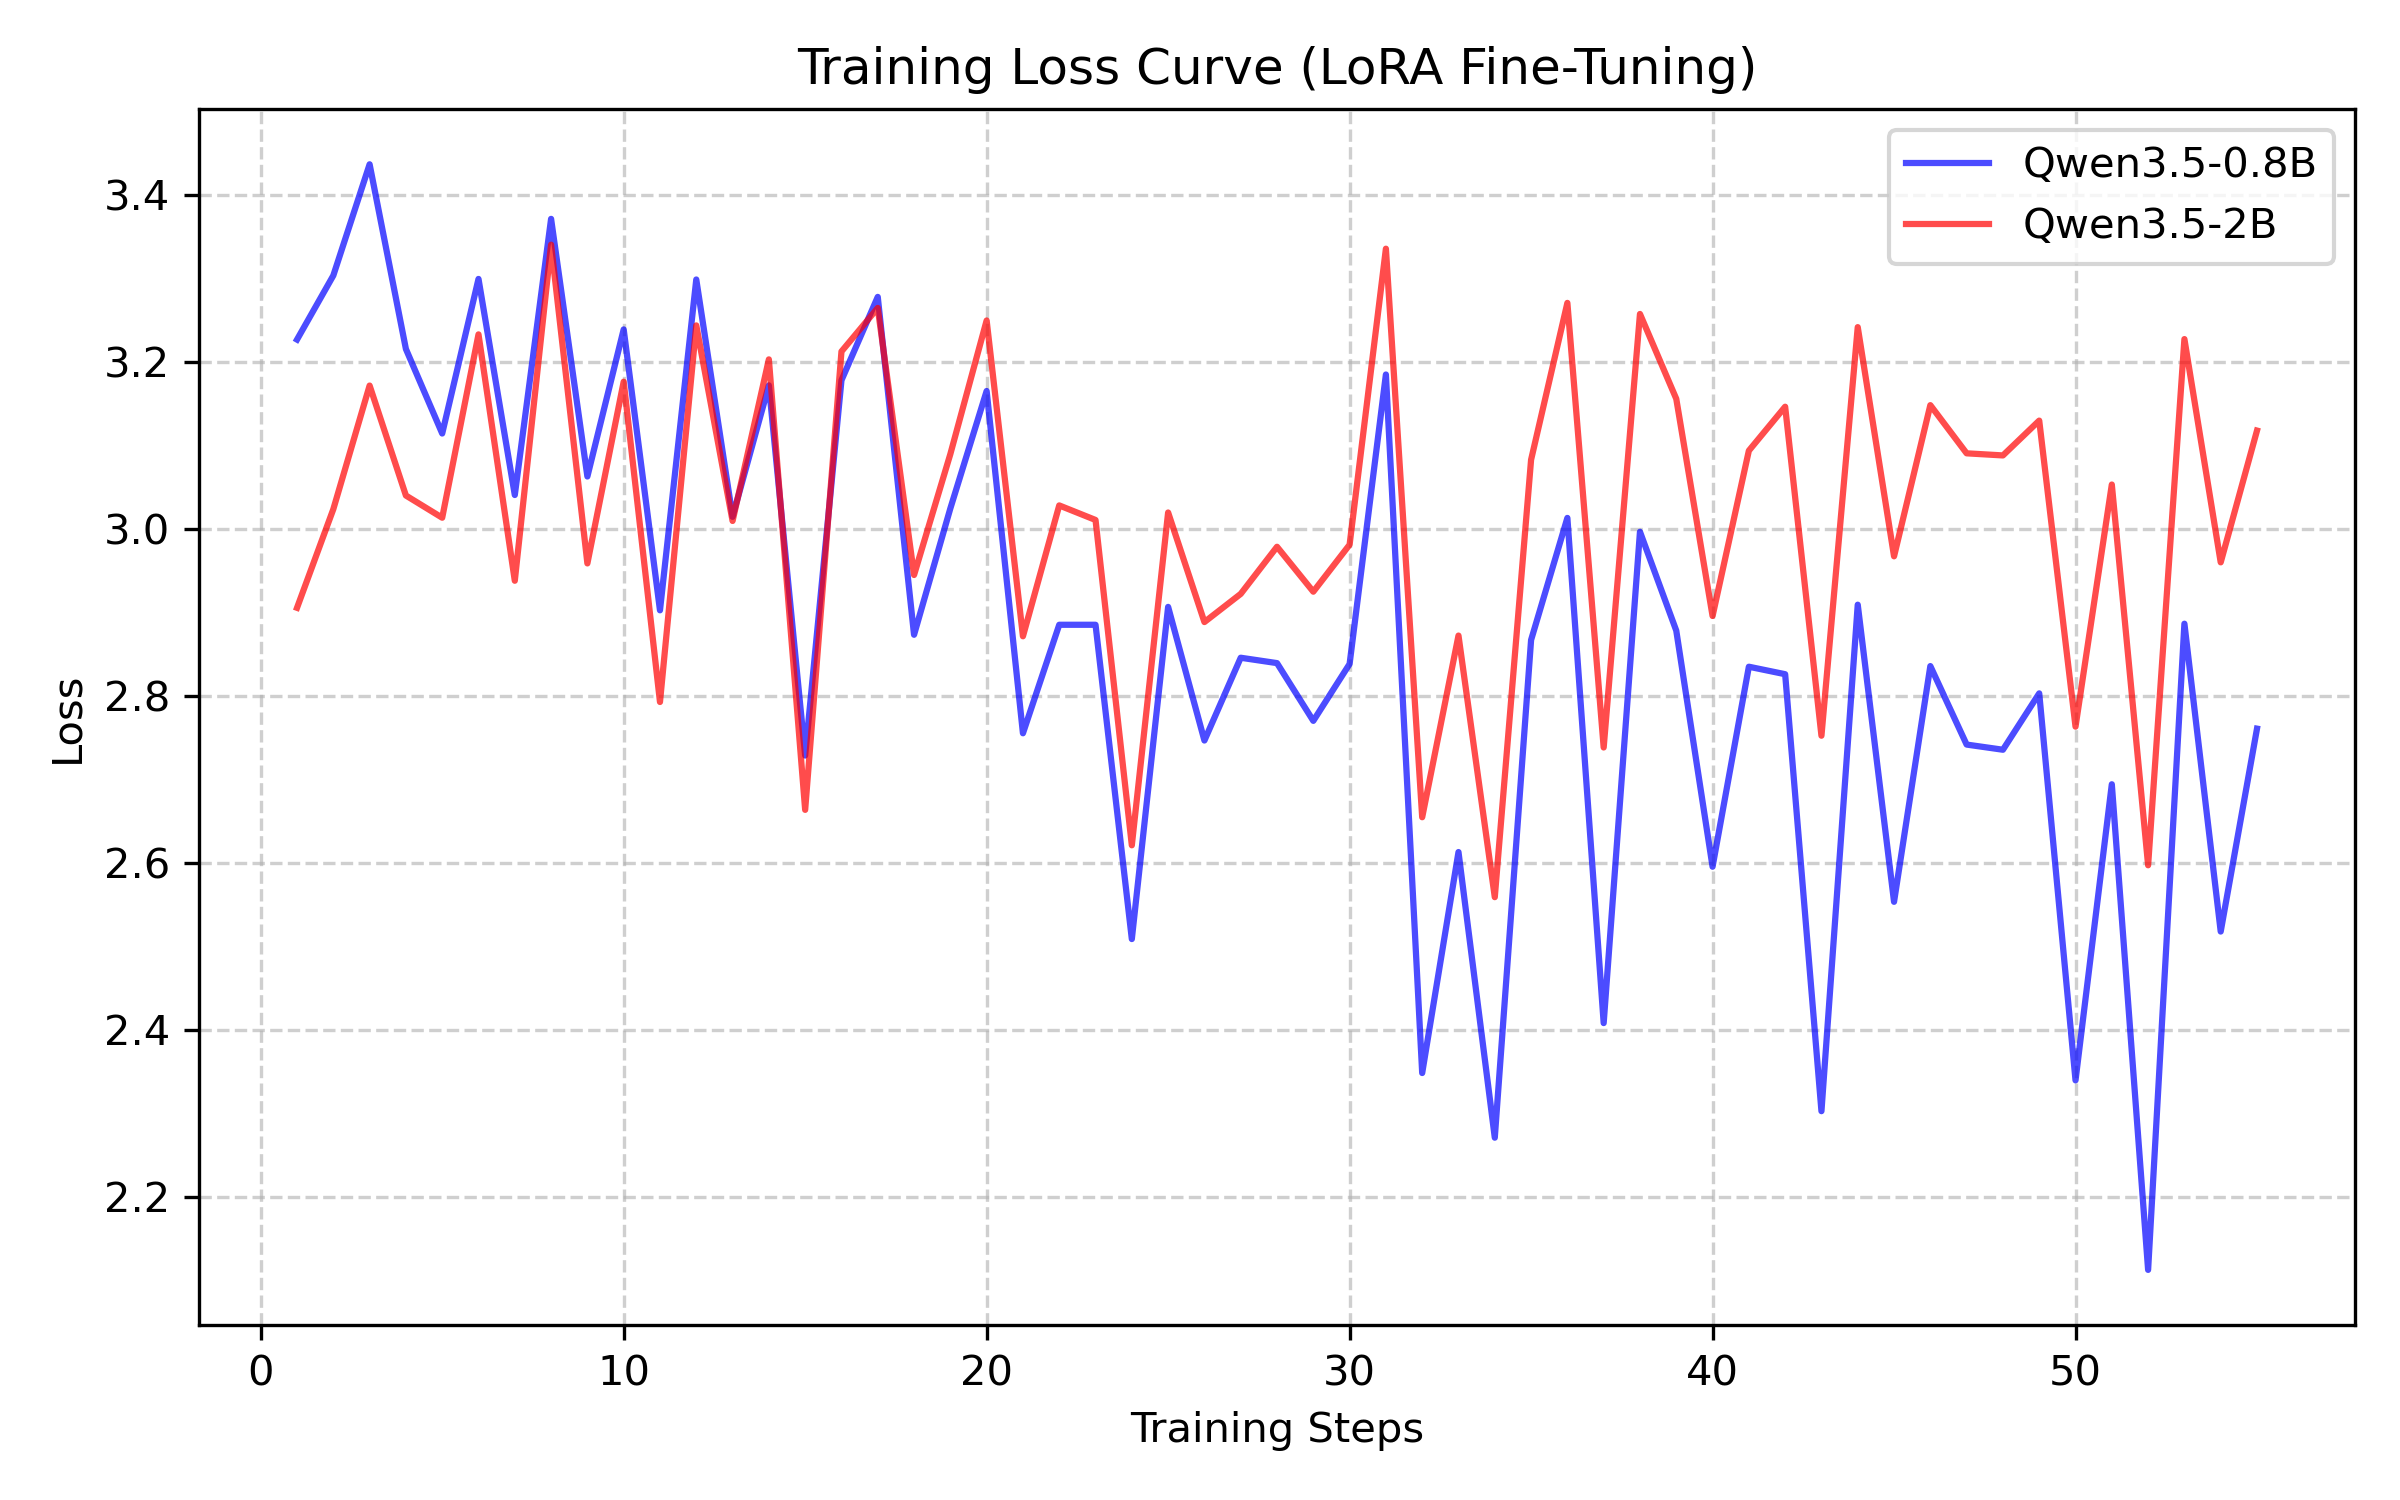
\includegraphics[width=0.8\linewidth]{images/training_loss.png}
    \caption{Training loss curves for Qwen3.5-0.8B and Qwen3.5-2B over one epoch (55 steps) of LoRA fine-tuning.}
    \label{fig:training_loss}
\end{figure}

\subsection{Extraction Performance}
Evaluation uses deterministic substring/soft-matching for semantic fields (\texttt{customer\_sector} and \texttt{customer\_scheduled\_at}) to handle terminology differences. Numerical variables are evaluated with both Mean Squared Error (MSE) to penalize large deviations and a $\pm 1$ accuracy tolerance to account for subjective human scaling.

\section{Discussion}
\label{sec:discussion}

\subsection{Obstacles and Strategies}

\subsection{What We Learned}

\subsection{Future Directions}

\section{Conclusion}
\label{sec:conclusion}

\bibliographystyle{oup-plain}
\bibliography{reference}

\end{document}
